\documentclass[11pt]{article}
\usepackage[utf8]{inputenc}
\usepackage{graphicx}
\usepackage{caption}
\usepackage{subcaption}
\usepackage{amsmath}
\usepackage{float}


\title{
	{Computer Vision 1 - Assignment 4 \\
	Image Alignment and Stitching}
}
\author{
Selene Baez Santamaria (10985417) - Andrea Jemmett (11162929)}
\date{\today}

\begin{document}

\maketitle

\section{Image alignment}
The main script for the image alignment is \texttt{alignment\_main.m}. To find
the affine transformation between the two given boat images we first computed their SIFT
descriptors and matches. To do this we used the \textit{VLFeat} toolbox which
exposed \texttt{vl\_sift} and \texttt{vl\_ubcmatch}; the former function accepts
an image as input and returns the identified keypoints and their SIFT
descriptors; the latter accepts two images as parameters and returns the indexes
ob matching keypoints in the two photoframes. As requested, we created a
function (\texttt{get\_matches.m}) that makes use of those functions and returns
the keypoints of both input images and their supposed matching ones.

We then use the \texttt{ransac.m} function that we created to find the best
parameters for the affine transformation using \textbf{RANSAC}. Our
implementation samples $P = 3$ pairs of matches (three points from the first
image and their three corresponding \textit{supposed} matches) at every
iteration, for a maximum of $N$ iterations. We implemented a sampling method in
\texttt{get\_sample.m}. Given that the transformation described in the
instructions requires six parameters and the following equations
\ref{eq:transform_point} and \ref{eq:transform_eq} to transform a point $(x,y)$
into $(x^{\prime}, y^{\prime})$:

\begin{equation}
	\label{eq:transform_point}
	A =
	\begin{bmatrix}
		x & y & 0 & 0 & 1 & 0 \\
		0 & 0 & x & y & 0 & 1
	\end{bmatrix}
	,\quad
	x =
	\begin{bmatrix}
		m_1 \\ m_2 \\ m_3 \\ m_4 \\ t_1 \\ t_2
	\end{bmatrix}
	,\quad
	b =
	\begin{bmatrix}
		x^{\prime} \\ y^{\prime}
	\end{bmatrix}
\end{equation}

\begin{equation} \label{eq:transform_eq}
	A x = b
\end{equation}

we noticed that by stacking the matrices $A$ for three points and the vectors
$b$ for their corresponding matches we could build a system of equations like
the following:

\begin{equation} \label{eq:affine_system}
	\begin{bmatrix}
		x_1 & y_1 & 0 & 0 & 1 & 0  \\
		0 & 0 & x_1 & y_1 & 0 & 1  \\
		x_2 & y_2 & 0 & 0 & 1 & 0  \\
		0 & 0 & x_2 & y_2 & 0 & 1  \\
		x_3 & y_3 & 0 & 0 & 1 & 0  \\
		0 & 0 & x_3 & y_3 & 0 & 1 
	\end{bmatrix}
	\begin{bmatrix}
		m_1 \\ m_2 \\ m_3 \\ m_4 \\ t_1 \\ t_2
	\end{bmatrix}
	=
	\begin{bmatrix}
		x^{\prime}_1 \\ y^{\prime}_1 \\ x^{\prime}_2 \\
		y^{\prime}_2 \\ x^{\prime}_3 \\ y^{\prime}_3
	\end{bmatrix}
\end{equation}

which consists of six unknown and six equations and so can be solved in Matlab
using \texttt{x = pinv(A)*b}.

At each iteration we transform the matched points in the first image and we plot
them over the second image. An example result is visible in Figure
\ref{fig:ransac_inliers}. Once we have the transformed points we can count the number of inliers,
defined as the number of transformed keypoints that fall under a distance of
10 pixels from their corresponding match in the second image.

\begin{figure}[htpb]
	\centering
	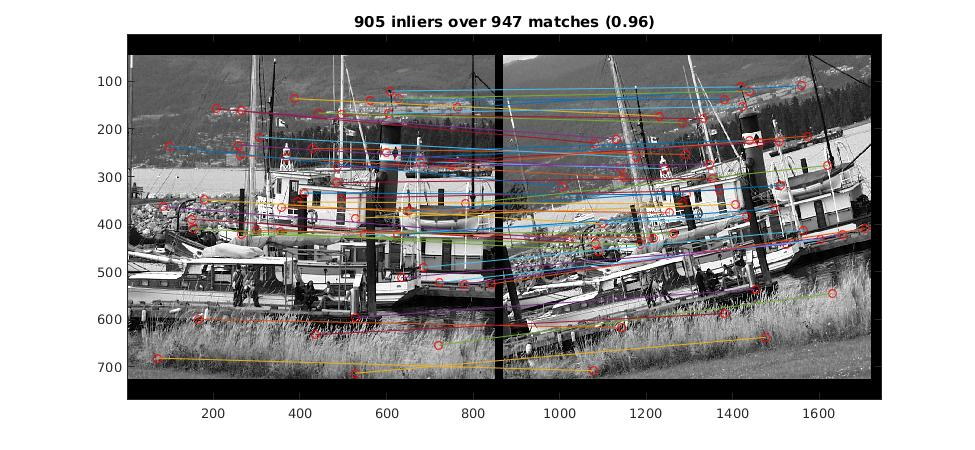
\includegraphics[width=1\textwidth]{imgs/transformed_matches.jpg}
	\caption{Each red dot is a keypoint and the lines connect keypoints that
	match. The keypoints on the right image are the keypoints of the left one, but
	transformed using the affine transformation during RANSAC; the algorithm finds
	a model that fits 905 inliers over 947 total matches.}
	\label{fig:ransac_inliers}
\end{figure}

If the count of inliers is greater than the one of the previous best iteration,
we store the transformation parameters and continue the loop. After $N$ loops
have been executed, the \texttt{ransac} function returns the best set of model
parameters, the count of inliers for each iteration and the keypoints sampled
that lead to the best parameters.

In Figure \ref{fig:aligned_im1} we show the first boat image transformed so to
match the alignment of the second boat image. Instead in Figure
\ref{fig:aligned_im2} we show the second boat image aligned to the first one
using the inverted transformation matrix.

\begin{figure}[htpb]
	\centering
	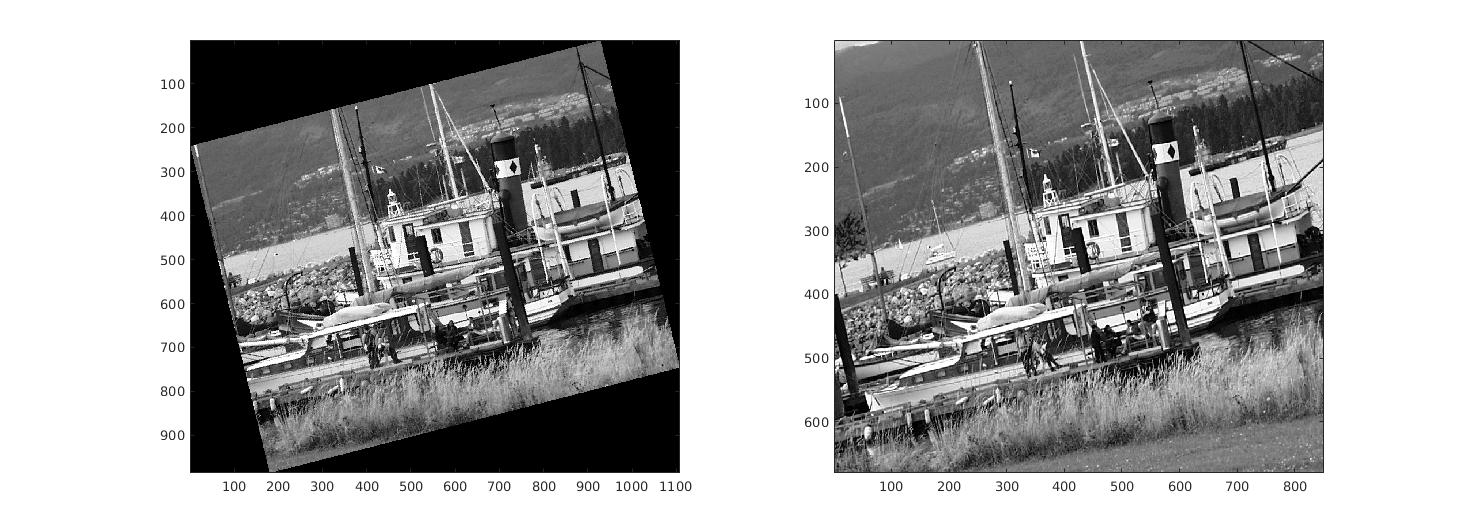
\includegraphics[width=1\textwidth]{imgs/aligned_im1.jpg}
	\caption{First boat image aligned to the second one.}
	\label{fig:aligned_im1}
\end{figure}

\begin{figure}[htpb]
	\centering
	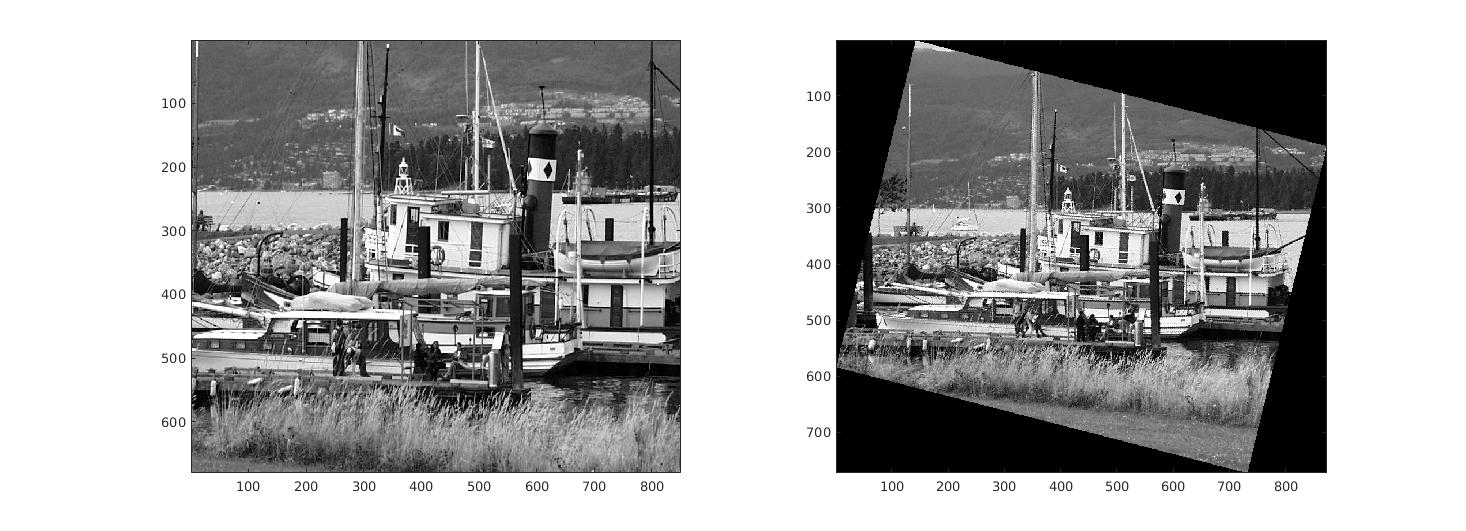
\includegraphics[width=1\textwidth]{imgs/aligned_im2.jpg}
	\caption{Second boat image aligned to the first one.}
	\label{fig:aligned_im2}
\end{figure}

By using the following formula we can compute how sufficiently big $N$ has to be
in order to have a likelihood of success, let's say, of $p = 0.99$.

\begin{equation}
	N > \frac{\ln(1 - p)}{\ln(1 - (1 - e)^P)}
	\label{eq:ransac_n}
\end{equation}

In equation \ref{eq:ransac_n} $p$ is the likelihood of success, $e$ is the
percentage of outliers (so $1 - e$ is the percentage of inliers) and $P$ is the
sample size ($P = 3$ in our case). Suppose we have $e = 0.5$, so that we expect
to encounter 50\% of outliers, we can plug in those values and find a minimum
value for $N$ that guarantees us to find the best set of parameters with a
probability of 99\%, which is $34.5$.

In Figure \ref{fig:imtransform_vs_custom} we show a comparison of the
transformed images using the function that we implemented (left column) and
Matlab's \texttt{imtransform} and \texttt{maketform} (right column). Both
functions implement nearest neighbor sampling and no differences are noticeable
by the naked eye. To transform the first image with the affine matrix, we first
find the size of the transformed image by computing minima and maxima (by
transforming the image corners with inverse warping, e.g. top-left, top-right,
bottom-left and
bottom-right) for each axis and then their difference. Then for each point $(x,
y)$ in the new image we compute the forward transformation of the $(x+x_{min},
y+y_{min})$ point and if it is in the boundaries of the image to be transformed,
we round it (so applying nearest neighbor interpolation) and put the value from
the image at that point into the new image at $(x, y)$, otherwise we put a zero.
To transform the second image and align it to the first one we use the same
function but applying a forward warping where we applied an inverse one and vice
versa. Our custom function can be found in \texttt{transform\_image.m}.

\begin{figure}[htpb]
	\centering
	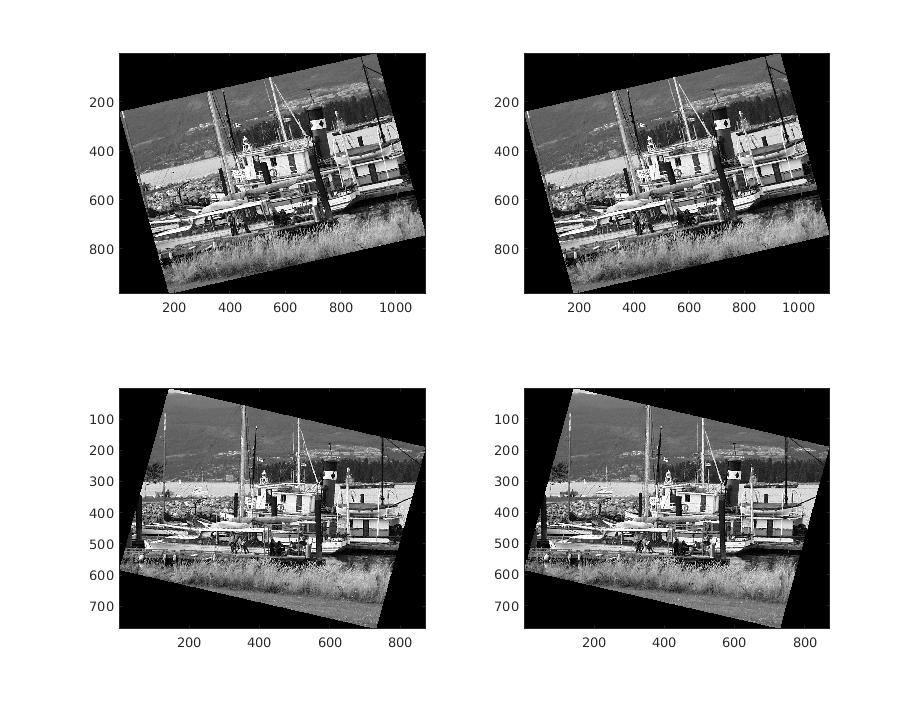
\includegraphics[width=1\textwidth]{imgs/imtransform_vs_custom.jpg}
	\caption{In the left column are the image transformed with the function
		\texttt{transform\_image.m} that we implemented. In the right
		column instead are the images transformed using Matlab's
		\texttt{imtransform}}.
	\label{fig:imtransform_vs_custom}
\end{figure}



\section{Image Stitching}
With the previously implemented functions we were able to create a stitching
function - which we called \texttt{stitch.m} - that takes two images and puts
them together in the same canvas to create a panorama. For demo purposes we used
the given images \textit{left.jpg} (as image 1) and \textit{right.jpg} (as image
2); a demo routine on these images can be found attached as
\texttt{stitching\_main.m}. Together they picture a bus on the street (Figure
\ref{fig:stitched}).

Firstly, since our functions work with gray scale values, we needed to transform
the input images from RGB to gray scale. Then we called the
\texttt{get\_matches.m} function to get the shared keypoints, and called
\texttt{ransac.m} to get the best transformation parameters, and the keypoints
that lead to those. The parameters for this were $N = 35$, $P = 3$, and $radius
= 10$.

Up to this point, the procedure was the same as for image alignment. However, in
order to put both images on the same canvas we need to find a shared coordinate
system that tells us where the shared points overlap. For this purpose we use
the set of keypoints returned by \textbf{RANSAC} on each image and average them
to produce what we called \textit{landmarks}.

Since the second image was in a space that was not yet comparable to the first
image, we first transformed the landmark to know where, in average, the
keypoints would lie. Additionally, we transformed the full image to the
equivalent space for image 1.

Given a landmark $L_1$ of the left image and the transformed landmark $L_2$ of
the right image, we compute the coordinates in which the second image should be
copied in the stitched image using the following formulae (origin is at top left):

\begin{equation}
	\begin{split}
		top &= L_{2y} - L_{1y} \\
		left &= L_{2x} - L_{1x} \\
		right &= width_{T(im2)} - L_{2x} - width_{im1} - L_{1x} \\
		bottom &= height_{T(im2)} - L_{2y} - height_{im1} - L_{1y}
	\end{split}
	\label{eq:stitch_corners}
\end{equation}

where $L_x$ and $L_y$ are the $x$ and $y$ coordinates of the landmark and
$T(im)$ is the transformed image. We proceed by estimating the size of the full
stitched image by means of the following equations:

\begin{equation}
	\begin{split}
		width_{stitch} &= width_{im1} + max(left, 0) + max(right, 0) \\
		height_{stitch} &= height_{im1} + max(top, 0) + max(bottom, 0)
	\end{split}
	\label{eq:estimate_stitch}
\end{equation}

In the final step, we need to place both images on the same canvas. We start by
copying the second image in, being careful of not falling outside the canvas
boundaries.

Secondly, we need to place the first image in the canvas. For this purpose we
calculate the space the full image 1 would need (named as
\textit{space\_needed}), and the available space the second image left (names as
\textit{space\_available}). Finally, we take the largest of the previous two
areas, and place it.

The final result is shown in Figure \ref{fig:stitched}.

\begin{figure}[htpb]
	\centering
	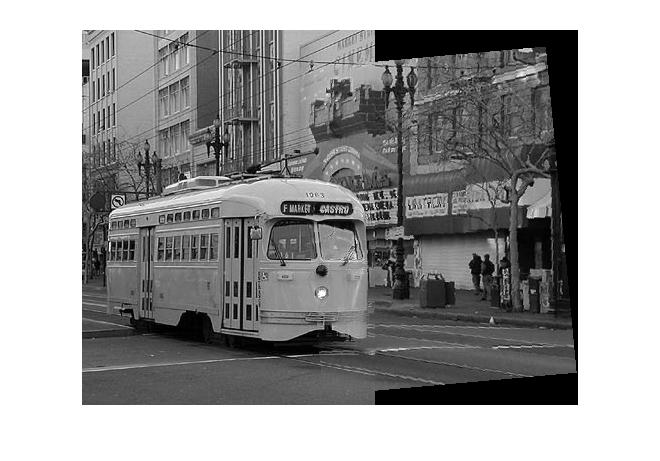
\includegraphics[width=1\textwidth]{imgs/stitched.jpg}
	\caption{Images \textit{left.jpg} and \textit{right.jpg} stitched in same
	panorama.}
	\label{fig:stitched}
\end{figure}


\end{document}
